\chapter{Results and Discussion}
\vspace{-1cm}
\section{Overview}

The current SwiftBite result is an interactive web prototype with a React-based customer experience and a separate Express API. The frontend demonstrates the principal screens of a food-ordering journey, while several operational integrations remain incomplete. This chapter presents current application screenshots and discusses what the implementation does and does not demonstrate.

\section{Current Application Outputs}
\vspace{-0.5cm}
\subsection{Landing Page and Customer Home}

The landing page introduces the SwiftBite service. The home screen includes restaurant cards, categories, offers, and popular dishes; the screenshot shows the promotion and food categories at the top of the page. Restaurant and menu content is bundled in frontend sample data rather than dynamically loaded from MySQL in the current customer flow.

\begin{figure}[H]
    \centering
    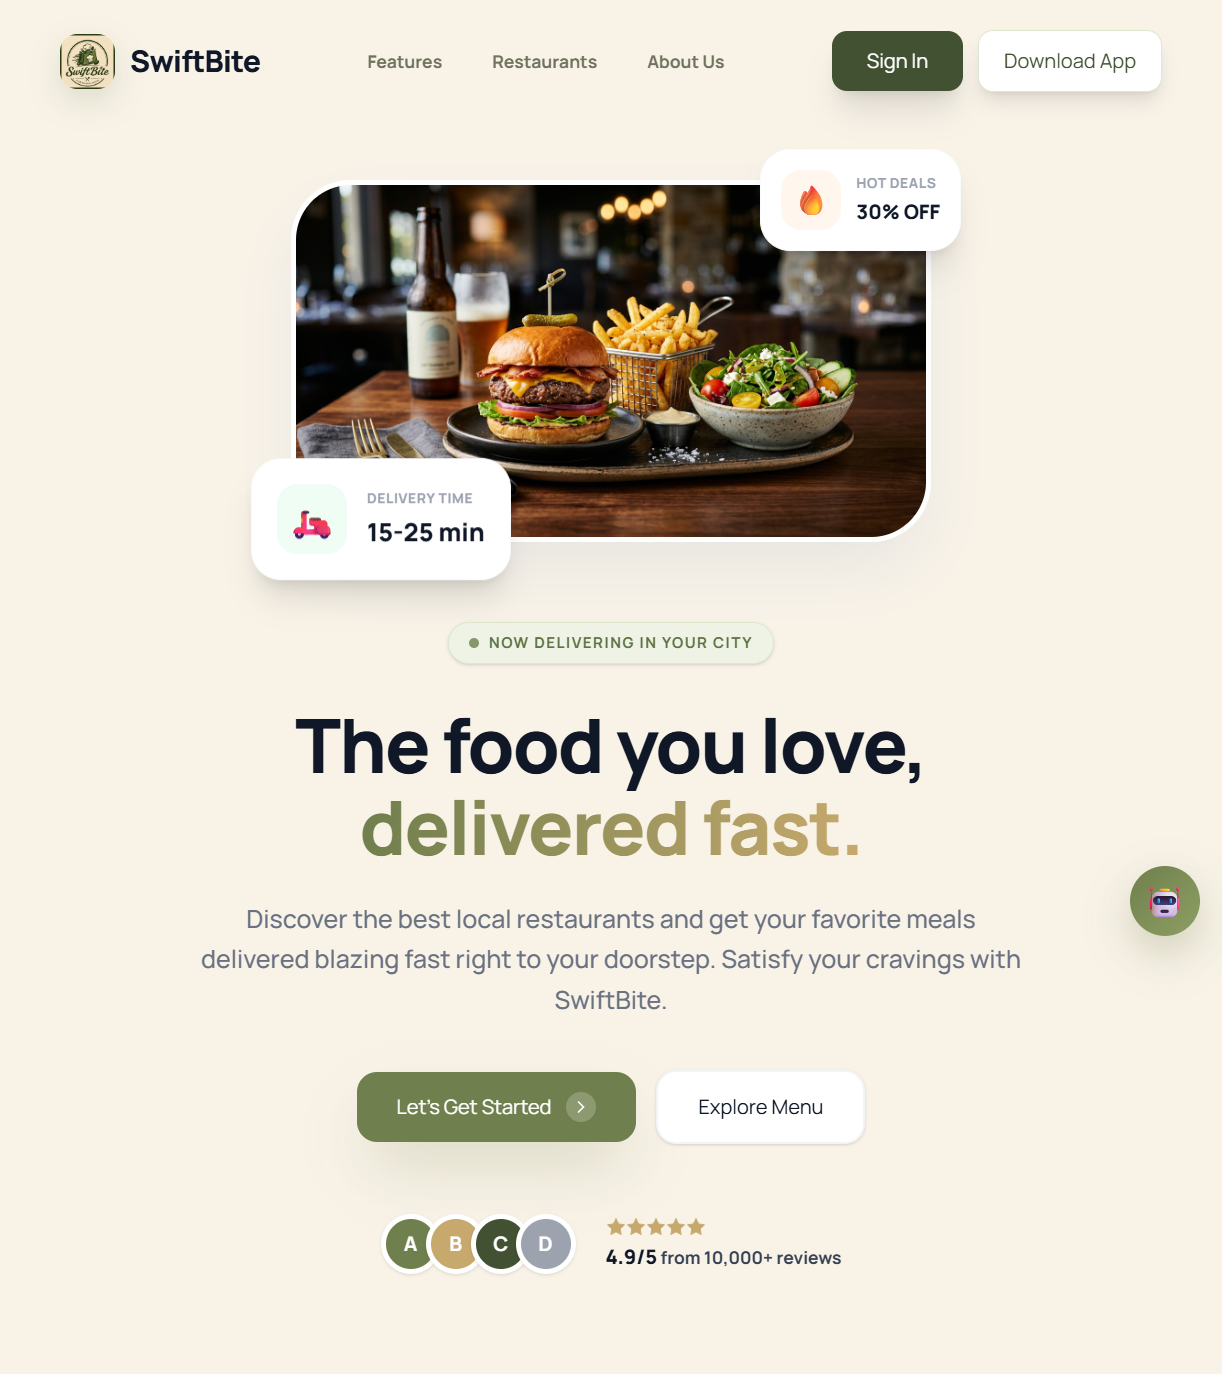
\includegraphics[width=0.9\textwidth,height=0.5\textheight,keepaspectratio]{Chapters/landing_page.png}
    \caption{Current SwiftBite landing page}
    \label{fig:result_landing}
\end{figure}

\begin{figure}[H]
    \centering
    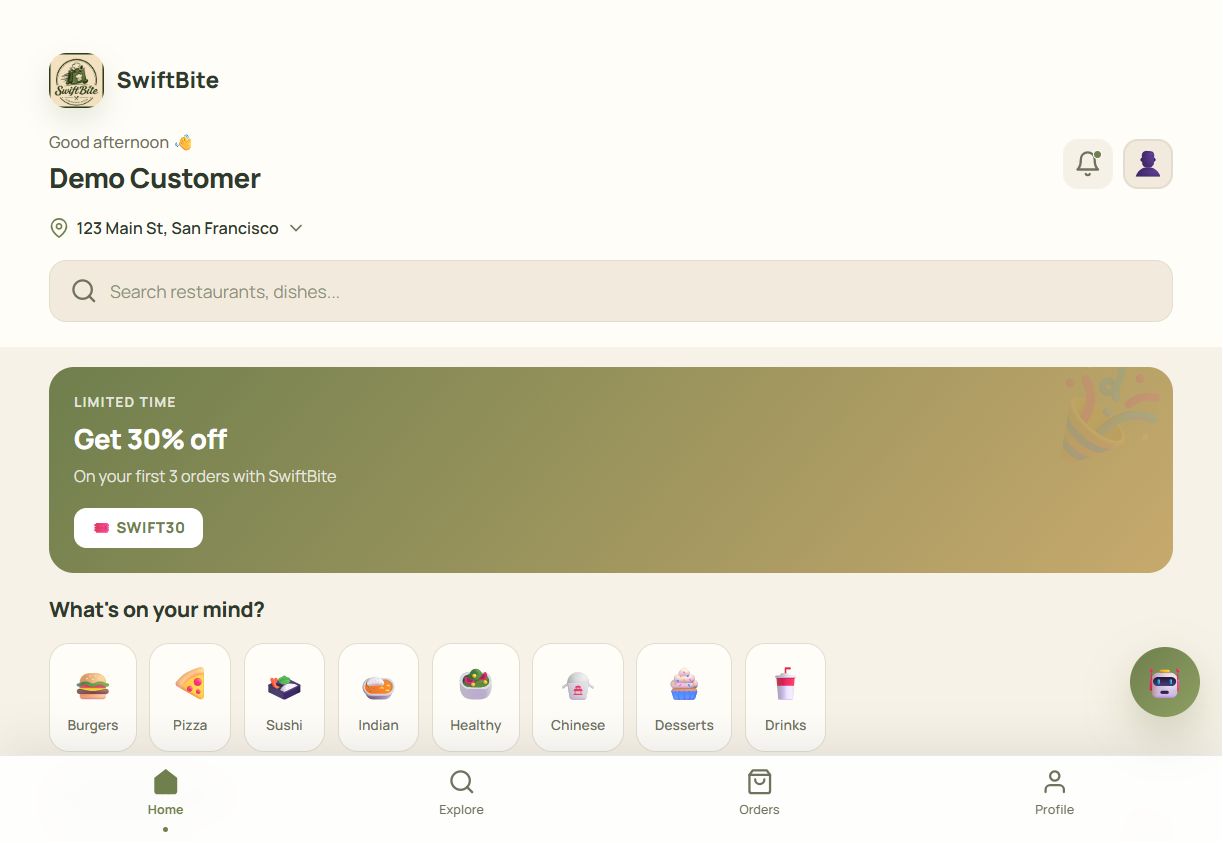
\includegraphics[width=0.9\textwidth,height=0.4\textheight,keepaspectratio]{Chapters/customer_home.png}
    \caption{Customer home screen showing the promotion and food categories}
    \label{fig:result_home}
\end{figure}

\subsection{Restaurant and Menu Browsing}

The restaurant detail screen displays a sample restaurant, category controls, menu items, and cart quantity actions. These interactions demonstrate the frontend workflow and use local state.

\begin{figure}[H]
    \centering
    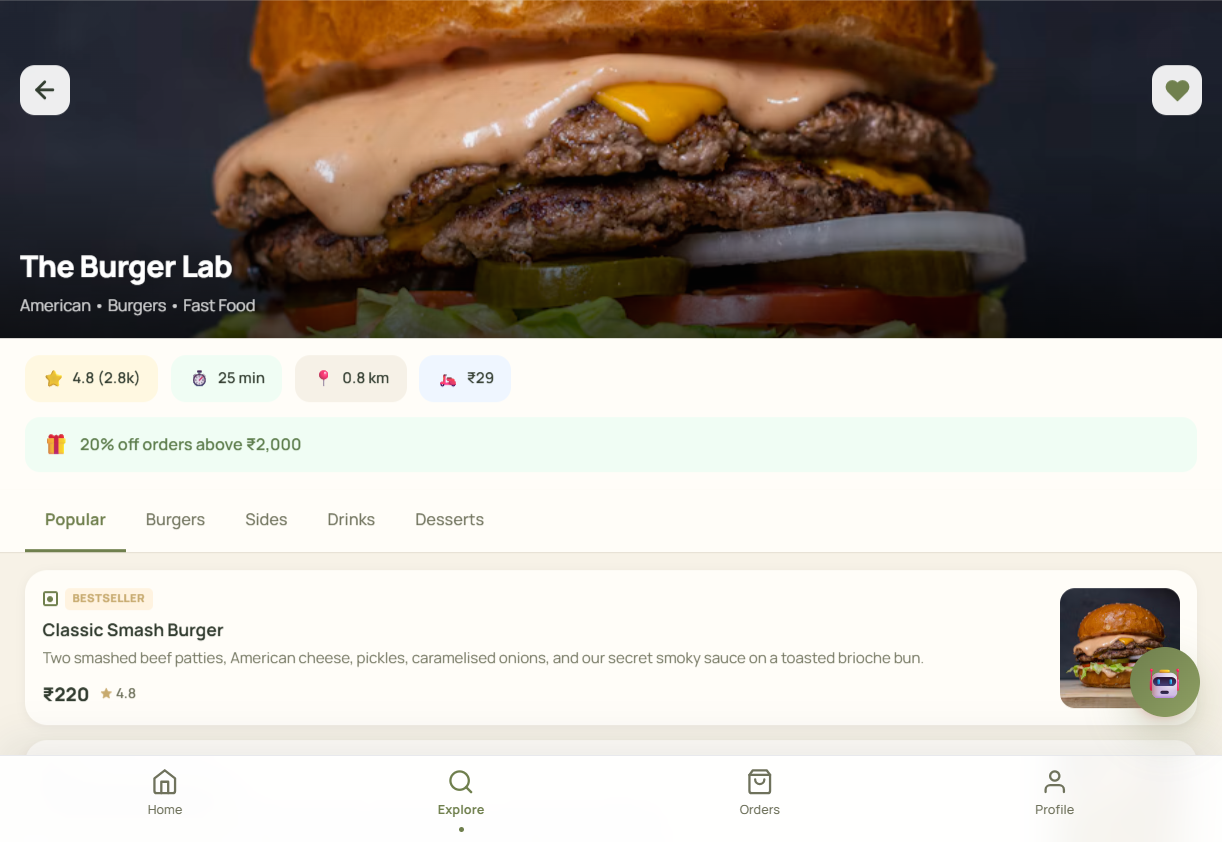
\includegraphics[width=0.9\textwidth,height=0.3\textheight,keepaspectratio]{Chapters/menu_list.png}
    \caption{Restaurant details and sample menu items}
    \label{fig:result_menu}
\end{figure}

\subsection{Account Registration}

The sign-up form accepts an email address or phone number and includes required password confirmation. The frontend checks that the password fields match before submitting; the backend registration schema also requires a matching confirmation value.

\begin{figure}[H]
    \centering
    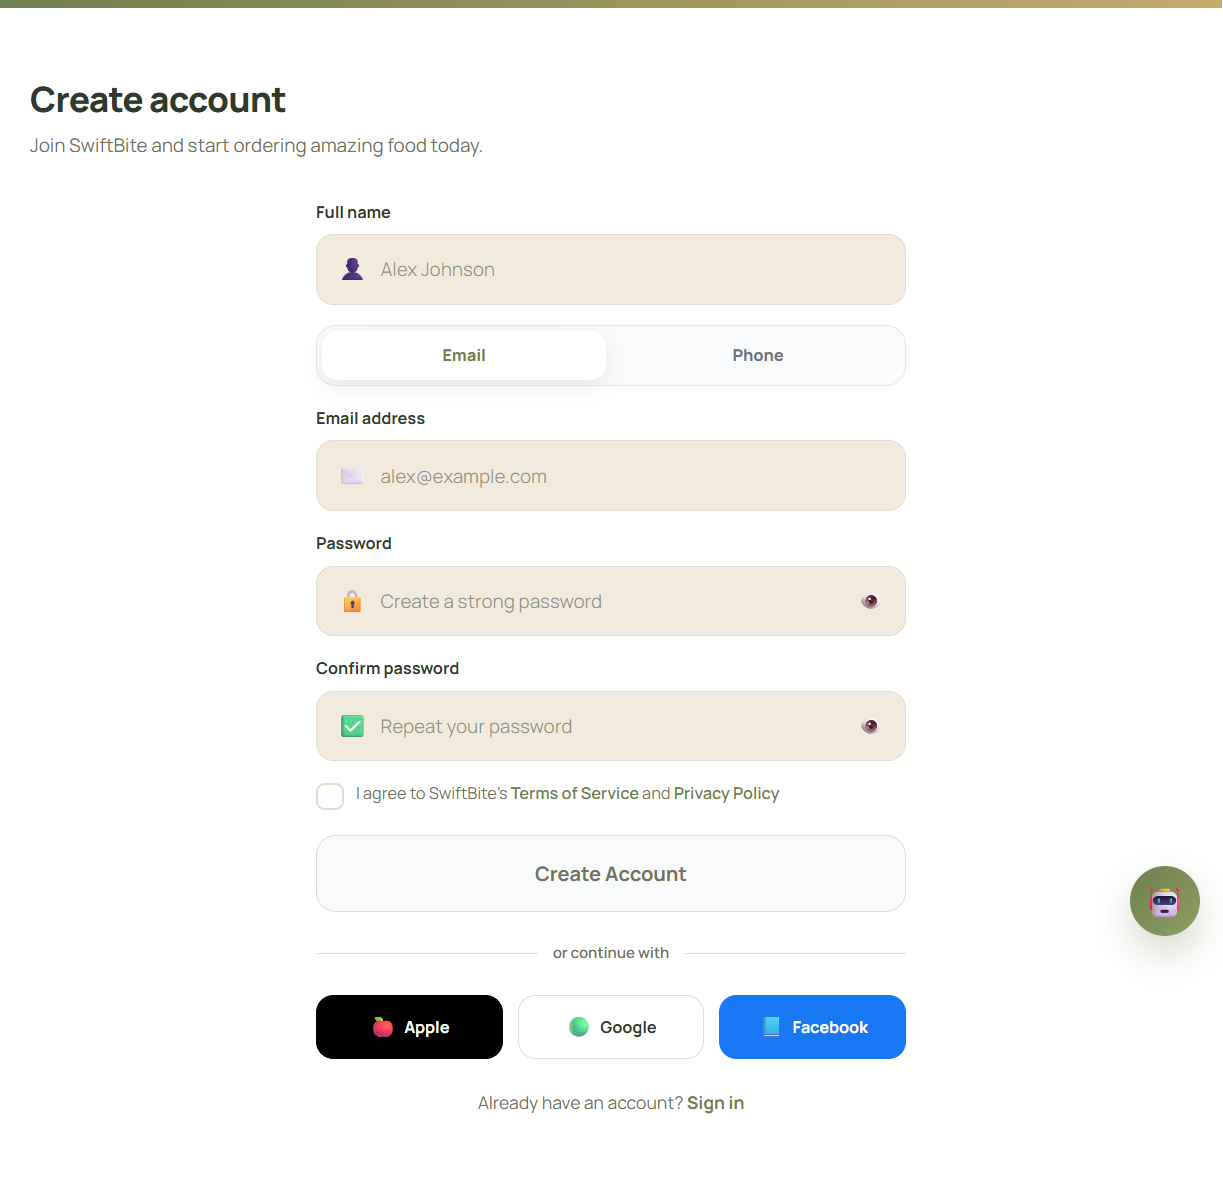
\includegraphics[width=0.72\textwidth,height=0.3\textheight,keepaspectratio]{Chapters/register.png}
    \caption{Current sign-up form with password confirmation}
    \label{fig:result_register}
\end{figure}

\subsection{Checkout and Order-Status Demonstrations}

The cart and checkout screens show quantity totals, delivery details, and payment choices. In the current frontend, selecting Place Order advances to a demonstration confirmation and order-status flow. It does not create a persistent order, process a payment, or retrieve live delivery coordinates.

\begin{figure}[H]
    \centering
    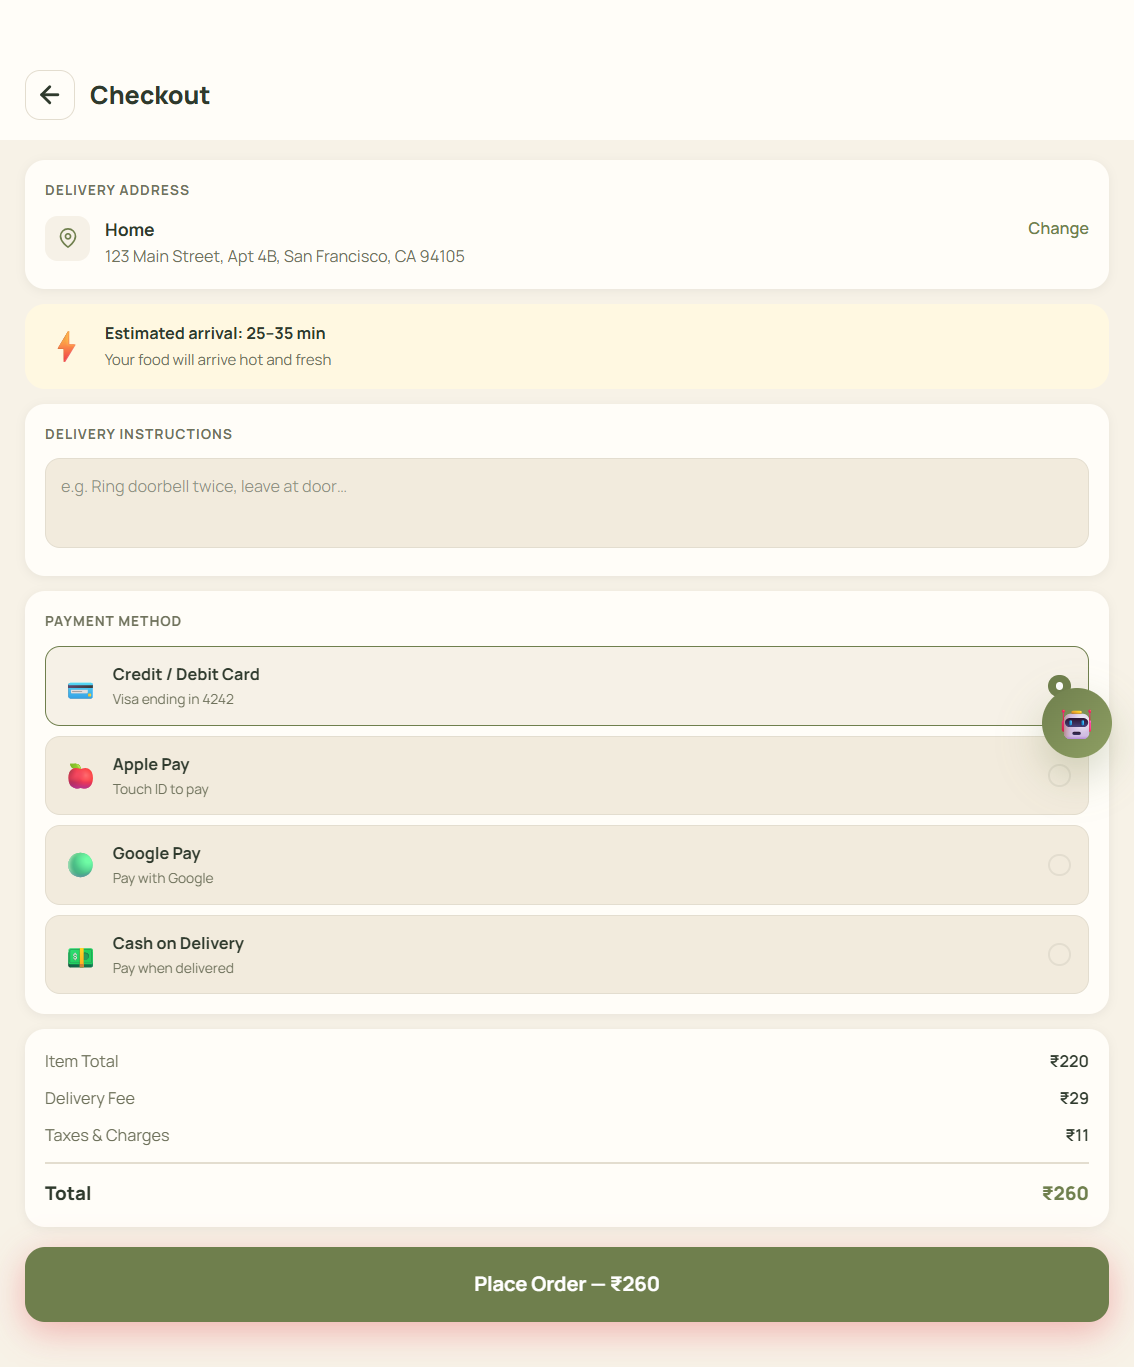
\includegraphics[width=0.9\textwidth,height=0.4\textheight,keepaspectratio]{Chapters/checkout.png}
    \caption{Checkout screen demonstrating delivery and payment selection}
    \label{fig:result_checkout}
\end{figure}

\begin{figure}[H]
    \centering
    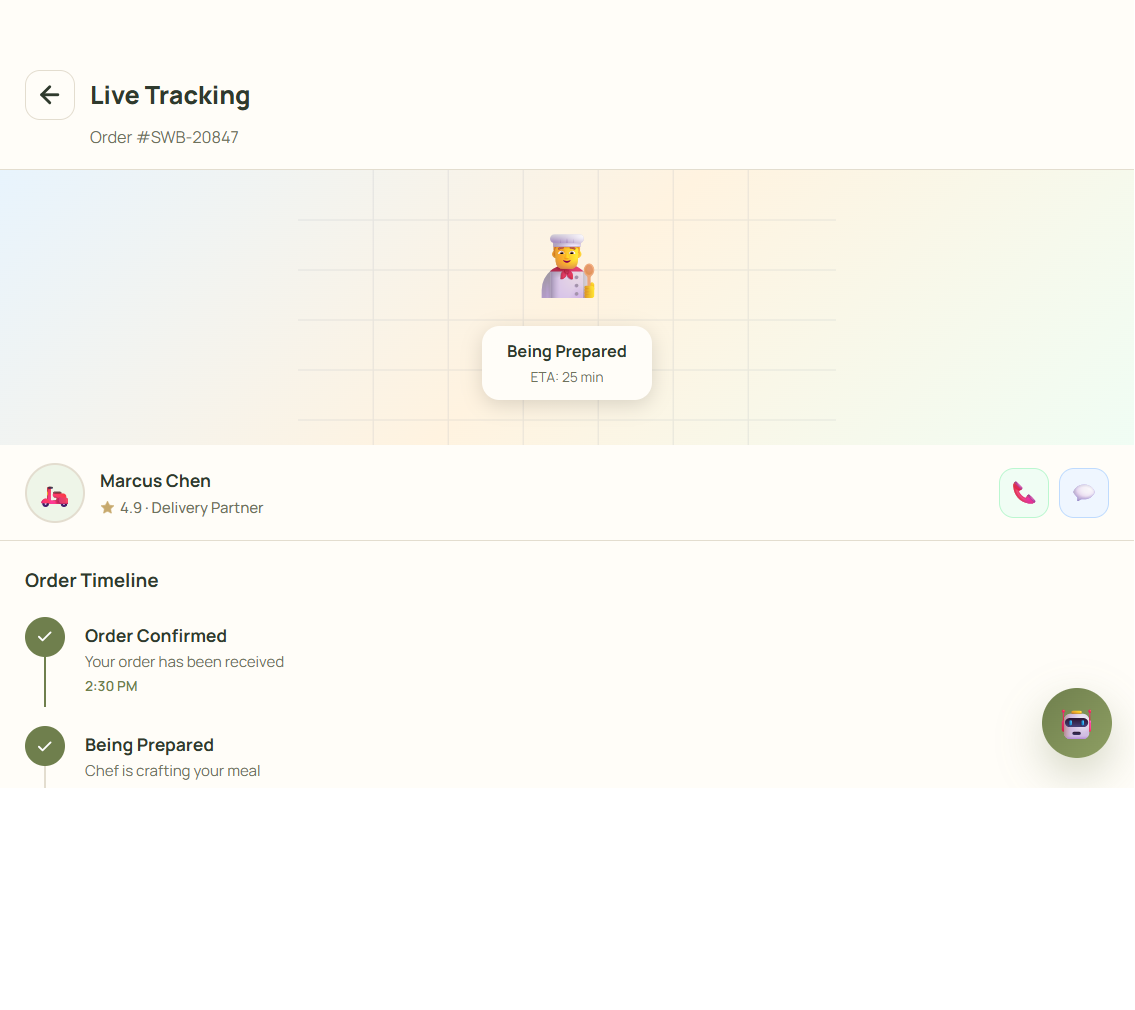
\includegraphics[width=0.9\textwidth,height=0.35\textheight,keepaspectratio]{Chapters/order_tracking.png}
    \caption{Demonstration order-status screen; not live GPS tracking}
    \label{fig:result_tracking}
\end{figure}

\subsection{Chatbot Assistance}

The chatbot responds to application questions. The frontend can use local rule-based responses when no API base URL is configured; the backend can call Gemini when its server-side key is present. The chatbot is an assistance feature and does not provide personalized food recommendations or place orders.

\begin{figure}[H]
    \centering
    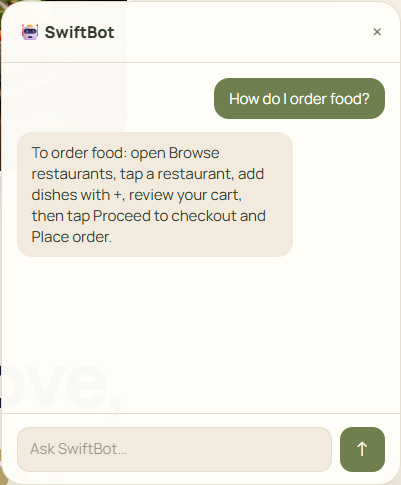
\includegraphics[width=0.9\textwidth,height=0.58\textheight,keepaspectratio]{Chapters/chatbot_test.png}
    \caption{Chatbot answering a food-ordering navigation question}
    \label{fig:result_chatbot}
\end{figure}

\section{Discussion of Findings}

\begin{itemize}
    \item \textbf{Frontend implementation:} React, TypeScript, and Vite provide a component-based interface. The customer catalogue and order journey currently use sample data and local state.
    \item \textbf{Backend capabilities:} The Express API includes authentication, profile, restaurant, menu, upload, order, dashboard, and chatbot routes. The storefront currently uses the authentication and chatbot services rather than integrating every available backend route.
    \item \textbf{Validation:} Zod validates backend request payloads. Registration requires password confirmation, and the frontend displays a mismatch error before sending the request.
    \item \textbf{Chatbot behavior:} Gemini is optional. Local rule-based responses allow app guidance without a configured model key or API base URL.
\end{itemize}

\section{Challenges and Current Constraints}

\begin{itemize}
    \item The frontend customer catalogue, cart, and checkout are not connected to persistent restaurant and order records.
    \item Payment methods are interface options only; there is no payment gateway or transaction processing.
    \item Order status is a demonstration screen and does not receive live events or GPS coordinates.
    \item Portal switching is demo functionality and does not enforce production server-side role authorization.
    \item The working MySQL connection, initialized schema, and database-backed restaurant API were verified. Full registration, login, and order-persistence integration tests remain outstanding; the file-backed authentication fallback is not a production persistence strategy.
\end{itemize}

\section{Summary}

SwiftBite currently demonstrates a responsive food-ordering interface, registration validation, a collection of backend API routes, and chatbot assistance. Its screenshots and results should be understood as prototype evidence. Persistent customer orders, real payment processing, live delivery tracking, and production-grade access control require further implementation and integration testing.
